\documentclass[11pt,fleqn]{article}
%\usepackage{CJK}
\usepackage{latexsym}
\usepackage{color}
\usepackage{graphicx, float}\usepackage{graphicx}
\usepackage{algorithmic}
\usepackage{algorithm}
%\usepackage{algpseudocode}
%\usepackage[colorlinks]{hyperref}
\usepackage[toc,page]{appendix}
\usepackage{bm}
\setlength{\oddsidemargin}{-0.0in}
\setlength{\evensidemargin}{-0.0in} \setlength{\textwidth}{6.0in}
\setlength{\textheight}{9.0in} \setlength{\topmargin}{-0.2in}
%\usepackage[boxruled]{algorithm2e}

%\setlength{\leftmargin}{0.7in}
\usepackage{amssymb, graphicx, amsmath}  %  fancyheadings,
\usepackage{setspace}
\newcommand\qed{\qquad $\square$}
\newcommand{\nn}{\nonumber}

\usepackage{lipsum}

\def \[{\begin{equation}}
\def \]{\end{equation}}
\def\proof{{\bf Proof:\quad}}
\def \endzm {\quad $\Box$}
\def\dist{\hbox{dist}}

\usepackage{tabularx,booktabs}
\newcolumntype{C}{>{\centering\arraybackslash\hsize=.5\hsize}X} % centered version of "X" type
\setlength{\extrarowheight}{1pt}
\usepackage{caption}% <-- added


\newcommand{\R}{\mathbb{R}}
%\newtheorem{yinli}{����}[section]
\newcommand{\D}{\displaystyle}
\newcommand{\T}{\textstyle}
\newcommand{\SC}{\scriptstyle}
\newcommand{\FT}{\footnotesize}

\usepackage{hyperref}
\newcommand\fnurl[2]{%
  \href{#2}{#1}\footnote{\url{#2}}%
}


%\newtheorem{theorem}{Theorem}[section]
%\renewcommand{\thetheorem}{\arabic{section}.\arabic{theorem}}
\newtheorem{definition}{Definition}
\renewcommand{\thedefinition}{\arabic{section}.\arabic{definition}}
\newtheorem{lemma}{Lemma}[section]
\renewcommand{\thelemma}{\arabic{section}.\arabic{lemma}}
\newtheorem{remark}{Remark}
\renewcommand{\theremark}{\arabic{section}.\arabic{remark}}
\newtheorem{proposition}{Proposition}[section]
\renewcommand{\theproposition}{\arabic{section}.\arabic{proposition}}
\newtheorem{corollary}{Corollary }[section]
\renewcommand{\thecorollary}{\arabic{section}.\arabic{corollary}}
\renewcommand{\theequation}{\arabic{section}.\arabic{equation}}
\renewcommand{\baselinestretch}{1.35}
\newtheorem{exam}{Example}[section]
\renewcommand{\theexam}{\arabic{section}.\arabic{exam}}
\newtheorem{theo}{Theorem}[section]
\renewcommand{\thetheo}{\arabic{section}.\arabic{theo}}

% Define a \HEADER{Title} ... \ENDHEADER block
\makeatletter
\newcommand{\HEADER}[1]{\ALC@it\underline{\textsc{#1}}\begin{ALC@g}}
\newcommand{\ENDHEADER}{\end{ALC@g}}
\makeatother

\newcommand{\argmin}{\operatornamewithlimits{argmin}}
\newcommand{\argmax}{\operatornamewithlimits{argmax}}

\begin{document}
%\begin{CJK*}{GBK}{song}

\begin{center}

{\LARGE \bf CS391L Machine Learning HW5: Reinforcement Learning}\\

\vskip 25pt
 {Zeyuan Hu, iamzeyuanhu@utexas.edu }\\
\vskip 5pt
{\small EID:zh4378 Fall 2017 }

\end{center}

\begin{spacing}{1.5}
\section{Introduction}

\paragraph{}In this task, we use the modular reinforcement learning (MRL) to explore a navigation task
in a 2D grid world of size $10\times10$, as shown in Figure 1. Our agent starts randomly on the left
side of the grid (denoted as \verb|start| in the figure) and its action space A = \{\emph{up}, \emph{down}, \emph{forward}\}.
There are \emph{objects} (orange square in the figure) that can be picked up, which leads to positive reward. In addition, there are 
\emph{litters} (red triangle) that cause negative reward when step onto it. Furthermore, the green cross represents \emph{exits}, which
give a large positive reward. The goal of the agent is to walk from the left side of the grid to the right side while
collecting as many objects as possible and trying his best to avoid litters. MRL divides the task into subtasks (modules)
and each module will learn its own policy using reinforcement learning. Then, module policies are combined to construct a global policy.
Concretely, we model each module as a Markov decision process (MDP), which is defined as a tuple $<S,A,T,R,\gamma>$ \cite{Sutton:1998}. Suppose
we have $n$ modules and $n$ corresponding MDPs $<S_1, A, T_1, R_1, \gamma_1>, \dots, <S_n, A, T_n, R_n, \gamma>$. Each module 
is trained with reinforcement learning and learned module policies $\pi_1, \dots, \pi_n$. Then, our job is to form a global policy
$\pi$ that maximize global reward based on module policies. In other words, we need to select a global action $a^*$ for 
global state $s$ based on the optimal actions $a_1, \dots, a_n$ proposed by each module based on their module states
$s_1, \dots, s_n$.

\begin{figure}[!b]
\centering
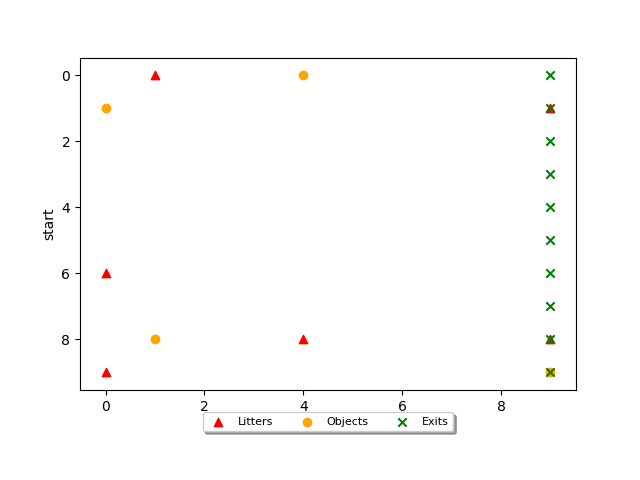
\includegraphics[scale=0.7]{environment.png} 
\caption{Environment}
\end{figure}

\section{Method}

\subsection{MRL}

MRL can be break down into three parts: decomposition, module training, and navigation and real-time global policy construction. 
For decomposition part, litters, objects, and exits form modules individually. The goal of agent for each module is defined as: avoiding
litters, picking up objects, and walking towards exits. Each module is modelled as a MDP independently. The state is defined as
the $(x,y)$ position in the grid and the action space $A$ is the same across all three modules. For module training part,
we train each module with Sarsa, which is defined as following:


\begin{algorithm}
  \caption{Sarsa}
  \begin{algorithmic}
	\STATE Let \textbf{s,a} be the original state and action, \textbf{r} is the reward observed in the following state, and
	$\boldsymbol{s',a'}$ are the new state-action pair.
	\STATE Initialize $\boldsymbol{Q(s,a)}$ arbitrarily
	\FOR{each episode}
	\STATE Initialize $\boldsymbol{s}$
	\STATE Choose $\boldsymbol{a}$ from $\boldsymbol{s}$ using policy derived from $\boldsymbol{Q}$
		   (i.e., $\epsilon$-greedy)
	\FOR {each step of episode}
	\STATE Take action $\boldsymbol{a}$, observe $\boldsymbol{r}, \boldsymbol{s'}$
	\STATE Choose $\boldsymbol{a'}$ from $\boldsymbol{s'}$ using policy derived from $\boldsymbol{Q}$ (i.e., $\epsilon$-greedy)
	\STATE $\boldsymbol{Q(s,a)} \leftarrow \boldsymbol{Q(s,a)} + \mu(\boldsymbol{r} + \gamma \boldsymbol{Q(s,a)} - \boldsymbol{Q(s,a)})$
	\STATE $\boldsymbol{s} \leftarrow \boldsymbol{s'}; \boldsymbol{a} \leftarrow \boldsymbol{a'}$
	\ENDFOR
	\ENDFOR
%    \HEADER{Forwards Pass}
%      \STATE Starting from the input layer, use eq.~\ref{update} to do
%      a forward pass trough the network, computing the activities of the
%      neurons at each layer.
%    \ENDHEADER
%    \HEADER{Backwards Pass}
%      \STATE Compute the derivatives of the error function with respect
%      to the output layer activities
%      \FOR{layer in layers}
%        \STATE Compute the derivatives of the error function with respect
%        to the inputs of the upper layer neurons
%        \STATE Compute the derivatives of the error function with respect
%        to the weights between the outer layer and the layer below
%        \STATE Compute the derivatives of the error function with respect
%        to the activities of the layer below
%      \ENDFOR
%      \STATE Updates the weights.
%    \ENDHEADER
\end{algorithmic}
\end{algorithm}

Intuitively, the agent will explore from state to state until it reaches either the step limit, which we specify in the
inner loop of the aglorithm, or the final state (i.e., exit). We call each exploration an episode. The major difference between 
Sarsa and Q-Learning is that the maximum reward for the next state is not necessarily used for updating the Q values. Instead, 
a new action, and therefore reward, is selected using the same policy that determined the original action. We keep the trained
Q table for each module.

For the navigation and real-time global policy construction part, at each global state $s$, our agent looks up
the Q values in each module for the given state $s$ and then we select a global action $a^*$ based on the global policy
construction algorithm and execute the action to move to a new global state $s'$. We implement three global policy
construction algorithms, which will be described in details in the following section.

\subsection{Global policy construction} 

The three algorithms are \emph{Module aggregation algorithm}, \emph{Module selection algorithm}, 
and \emph{Module voting algorithm} \cite{Zhang:2015}.

\begin{itemize}
\item \textbf{Module aggregation algorithm} selects the action that maximizes the Q value of all modules combined for a given state.
Concretelym we choose action $a^* = \argmax_a Q(s,a)$, where $Q(s,a) = \sum_i Q_i(s_i,a)$ with $i$ representing module $i$.
\item \textbf{Module selection algorithm} selects the action that has the highest weight across the all modules. Let $W_i(s_i)$ denote
the weight of module $i$ at state $s_i$. We choose $W_i(s_i) = \sigma(Q_i(s_i,a))$, where $\sigma(Q_i(s_i,a))$ is the standard
deviation of Q values acorss actions. The intuition behind the scene is that the variance of Q values across all actions indicates
how indifferent the module is about its action selection. Large variance indicates that choosing different ations lead to very different
expected reward.
\item \textbf{Module voting algorithm} selects the action that has highest votes. Let $K(s_i, a)$ be vote count for global action $a$,
then $K(s_i, a) = \sum_iW_i(s_i)$ for all module $i$ whose optimal action $a_i = a$. In other words, each module $i$ put
$W_i(s_i)$ votes on its optimal action $a_i$. Global action is selected as the action with highest number of votes $a^* = \argmax_aK(s_i,a)$.
\end{itemize}


\subsection{Implementation}

We use \verb|REWARD_EMPTY|, \verb|REWARD_OBJ|, \verb|REWARD_LITTER|, and \verb|REWARD_EXIT| to denote
the rewards for empty grid, objects, litters, and exits respectively, which are initialized to 0, 5, -4, and 100.
Functions \verb|avoidLittersReward|, \verb|pickingObjsReward|, and \verb|exitingMapReward| are used to generate
the reward matrix for avoiding litters, picking up objects, and walking towards exit modules individually. Each reward
matrix is generated independently and thus litters, objects, and exits can appear simultaneously in the same cell.
In addition to reward matrix, we also generate the cell state matrix (i.e., \verb|R_state|), which is to keep track
of the states of the cells of the grid. There are four possible states: \verb|L|, \verb|O|, \verb|X|, and \verb|E|,
which represents that the cell has ``Litters", ``Objects", ``Exits", or nothing. The purpose for the state matrix
is that the litters or the objects can be stepped onto once and we need to change the reward once the agent passes those
cells.

Sarsa algorithm is implemented as \verb|sarsa| that takes in reward matrix \verb|R|, state matrix \verb|R_state|, a 
set of hyperparameters including $\mu$, $\gamma$, $\epsilon$, numEpisode, and numSteps. The implementation follows
closely to the algorithm stated above. The output of the algorithm is the trained Q table. \verb|drawGrid| contains
all three global policy construction algorithms, the action execution based on the global policy, and the plotting
of the grid and the agent exploration route. \verb|drawGrid| takes in the Q table(s), reward matrices, maximum number of
steps that agent can move, mode, policy, 
and a boolean \verb|checkRepeatActions|. The input Q table and reward matrices have to be packed as a list of 
Q table matrix and reward matrix resepectively. This allows us to use one single \verb|drawGrid| function to handle
all possible cases: avoiding litters module only, picking up objects only, walking towards the exit only, and 
all three modules combined. Which module we are working with is specified with \verb|mode|. Accepted values ranged
from 0 to 3 inclusive to indicate avoiding litters module, picking up objects, walking towards the exit, and all three
modules combined. \verb|policy| variable specifies which global policy construction we want to use and \verb|checkRepeatActions|
specifies whether we want to detect the repeative actions, which is shown in figure 2. Once the agent moves to the cell
$[0,1]$, the optimal global action keeps instructing the agent to go up, which is not possible. Thus the agent stays
at the original place and stay here forever (the path of agent is shown in blue). To handle case like this, we invent a protocol that randomly select the action
to execute when we detect there have been repeat actions in the past using \verb|checkCycle| function. The impact of 
\verb|checkRepeatAction| is shown in figure 3.

\begin{figure}
\centering
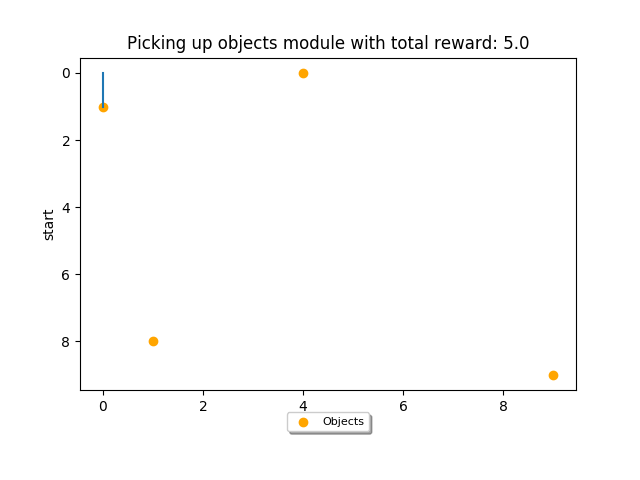
\includegraphics[scale=0.7]{repeatActions.png} 
\caption{checkRpeatActions=False for picking up objects module}
\end{figure}

\begin{figure}
\centering
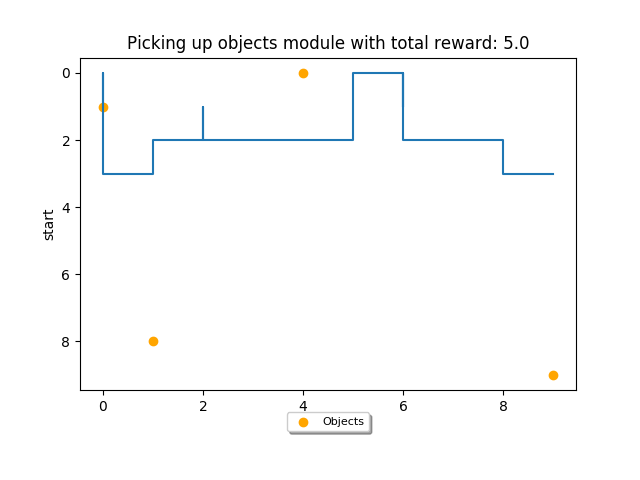
\includegraphics[scale=0.7]{noRepeatActions.png} 
\caption{checkRpeatActions=True for picking up objects module}
\end{figure}

\section{Results}

Without specific note, we use the hyperparameters shown in the table 1. The heuristic 
for setting up the discount factor $\gamma$ for each module is that we want to prioritize
walking towards exits goal. In general $\gamma$ has a range of 0 to 1. If $\gamma$ is closer
to zero, the agent will tend to consider only immediate rewards. If $\gamma$ is closer to one,
the agent will consider future rewards with greater weight, willing to delay the reward.

\begin{table}
\captionsetup{size=footnotesize}
\caption{Hyperparameter configuration for the navigation task} \label{tab:freq}
%\setlength\tabcolsep{0pt} % let LaTeX compute intercolumn whitespace
\footnotesize\centering
%This table provides the frequencies.

\smallskip 
\begin{tabular*}{\columnwidth}{@{\extracolsep{\fill}}lc}
\toprule
  Description  & Values  \\
\midrule
 grid width & 10      \\
 grid length & 10 \\
 number of litters & 10        \\
 number of objects & 4        \\
 $\mu$ & 0.7        \\
 $\epsilon$ & 0.5 \\
 numEpisode (module training) & 200 \\
 numSteps (module training) & 100 \\
 maximum number of steps that agent can move & 200 \\
 $\gamma$ for avoiding litters & 0.4 \\
 $\gamma$ for picking up objects & 0.7 \\
 $\gamma$ for walking towards exit & 1 \\
\bottomrule
\end{tabular*}
\end{table}

The performance of each individual module given \verb|checkRepeatActions=True| is shown 4, 5, and 6.
The performance for picking up objects module is shown in Figure 2 above. Additional plots of all three modules
combined can be seen in the appendices.

\begin{figure}
\centering
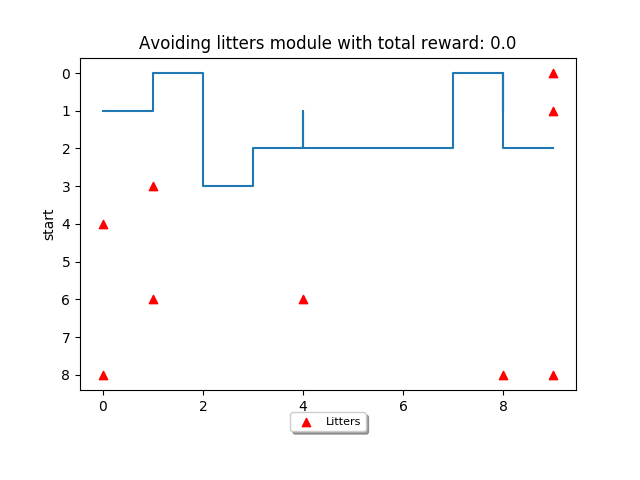
\includegraphics[scale=0.7]{avoidingLitters.png} 
\caption{Performance of avoiding litters module}
\end{figure}

\begin{figure}
\centering
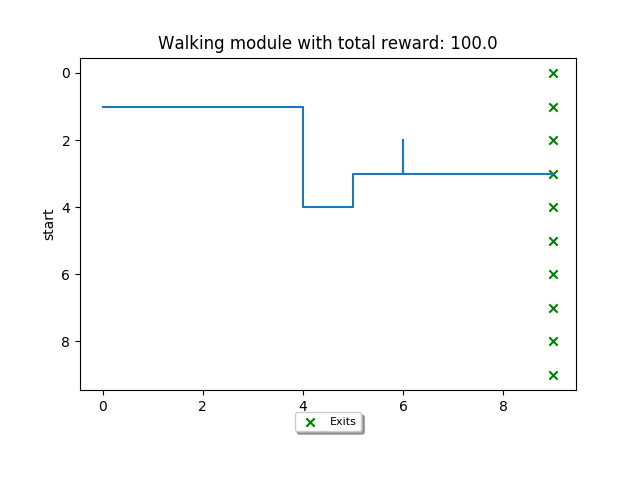
\includegraphics[scale=0.7]{walkingTowardsExits.png} 
\caption{Performance of walking towards exits module}
\end{figure}

\begin{figure}
\centering
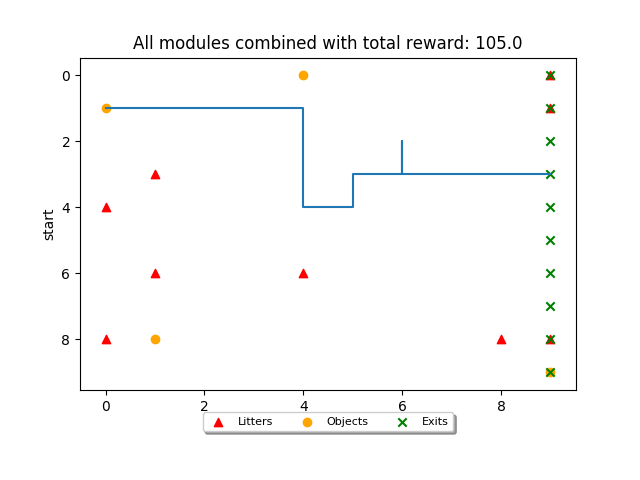
\includegraphics[scale=0.7]{combined.png} 
\caption{Performance of all three modules combined}
\end{figure}

We also experiment with the efficiency of the global policy construction algorithm by measuring how many
steps that the agent has to perform in order to reach the exits and the total reward collected in the end. 
For this experiment, we change the following
hyperparameters shown in table 2. The rest of hyperparameters are kept untouched.

\begin{table}
\captionsetup{size=footnotesize}
\caption{Hyperparameter configuration for globlal policy construction algorithms} \label{tab:freq}
%\setlength\tabcolsep{0pt} % let LaTeX compute intercolumn whitespace
\footnotesize\centering
%This table provides the frequencies.

\smallskip 
\begin{tabular*}{\columnwidth}{@{\extracolsep{\fill}}lc}
\toprule
  Description  & Values  \\
\midrule
 grid width & 100      \\
 grid length & 100 \\
 number of litters & 30        \\
 number of objects & 40        \\
 maximum number of steps that agent can move & 1000 \\
\bottomrule
\end{tabular*}
\end{table}

The performance of using \emph{module voting algorithm} is shown in Figure 7 and 
the performance of using \emph{module aggregation algorithm} is shown in Figure 8.

\begin{figure}
\centering
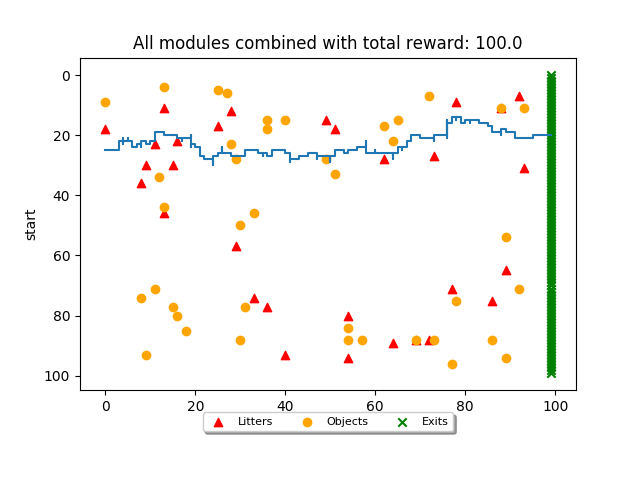
\includegraphics[scale=0.7]{module_voting_algorithm.png} 
\caption{Performance of all three modules combined with module voting algorithm}
\end{figure}

\begin{figure}
\centering
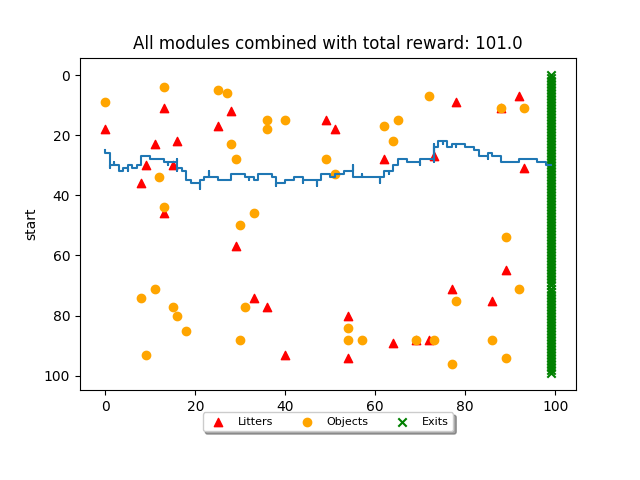
\includegraphics[scale=0.7]{module_aggregation_algorithm.png} 
\caption{Performance of all three modules combined with module aggregation algorithm}
\end{figure}

Table 2 summarizes the performance of three global policy construction algorithms measured by
the number of steps used and the total reward collected. As shown in the table, all three algorithms
do not make fundamentally difference. However, module aggregation algorithm works better than the other
two algorithms in terms of total rewards collected. In addition, the peformance of algorithms stay
the same no matter whether we turn on \verb|checkRepeatActions| or not during the training phase of each
module.

\begin{table}
\captionsetup{size=footnotesize}
\caption{Performance of globlal policy construction algorithms} \label{tab:freq}
%\setlength\tabcolsep{0pt} % let LaTeX compute intercolumn whitespace
\footnotesize\centering
%This table provides the frequencies.

\smallskip 
\begin{tabular*}{\columnwidth}{@{\extracolsep{\fill}}lcc}
\toprule
  Algorithm  & Number of Steps & Total Rewards  \\
\midrule
 module aggregation algorithm & 264 & \textbf{101}      \\
 module selection algorithm & 264 & 100 \\
 module voting algorithm & 264 & 100        \\
\bottomrule
\end{tabular*}
\end{table}

We also experiment with the impact of the discount factor $\gamma$ onto the agent's performance.
We vary the discount factor for walking towards the exits module and measure the number of steps
and total rewards collected. The hyperparameters configuration is the same with the previous experiment
except that now we vary $\gamma$ from $0$ to $1$ with $0.1$ intervals (i.e., $0, 0.1, 0.2, \dots, 1$).
We use \emph{module voting algorithm} and turn off \verb|checkRepeatActions| during the training phase 
for this experiment. The performance of the agent is summarized in table 3. 

\begin{table}
\captionsetup{size=footnotesize}
\caption{Performance of globlal policy construction algorithms} \label{tab:freq}
%\setlength\tabcolsep{0pt} % let LaTeX compute intercolumn whitespace
\footnotesize\centering
%This table provides the frequencies.

\smallskip 
\begin{tabular*}{\columnwidth}{@{\extracolsep{\fill}}lcc}
\toprule
 $\gamma$  & Number of Steps & Total Rewards  \\
\midrule
 0   & 260 & \textbf{105}  \\
 0.1 & 260 & \textbf{105}  \\
 0.2 & 260 & \textbf{105}  \\
 0.3 & 264 & 96   \\
 0.4 & 264 & 96   \\
 0.5 & 264 & 96   \\
 0.6 & 264 & 96  \\
 0.7 & 264 & 96  \\
 0.8 & 265 & \textbf{105}  \\
 0.9 & \textbf{262} & 100  \\
 1.0 & 264 & 100  \\
\bottomrule
\end{tabular*}
\end{table}

The importance of \verb|checkRepeatActions| protocol becomes apparent when we deal with large grid in
this case. Figure 9 shows the result of the agent exploration after $1000$ steps. As shown in the figure,
the agent cannot fully explore the space and fail to reach the exits given the step constraint.

\begin{figure}[!b]
\centering
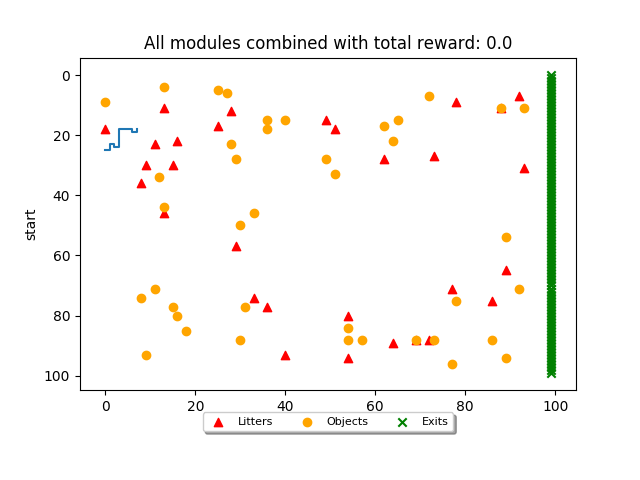
\includegraphics[scale=0.7]{noRepeatActions_large.png} 
\caption{checkRpeatActions=False for three modules combined with 1000 maximum number of steps}
\end{figure}

\section{Conclusion}

In this task, we implement MRL and apply it towards the navigation task. We implement three
global policy construction algorithms and show the effectiveness of the algorithms for the given task.
In addition, we explore the impact of the discount factors on the agent's performance and demonstrate
the importance of \verb|checkRepeatActions| protocol on achieving desirable task outcome.

\end{spacing}

\bibliographystyle{ieeetr}
\bibliography{report}

\begin{appendices}

\section{How to run the code}

\paragraph{}To run my code, unzip the \verb|hw5.zip| and get \verb|rl.py|. Then, you
can run the code with the following commands:

\begin{itemize}
\item \verb|python rl.py L| Run the MRL on avoiding litters module only
\item \verb|python rl.py O| Run the MRL on picking up objects module only
\item \verb|python rl.py X| Run the MRL on walking towards exit module only
\item \verb|python rl.py A| Run the MRL on all three modules combined
\end{itemize}

My code is heavily commented and please take a look if there are any type of questions.

\section{Additional plots of agent explorations}

\begin{figure}
\centering
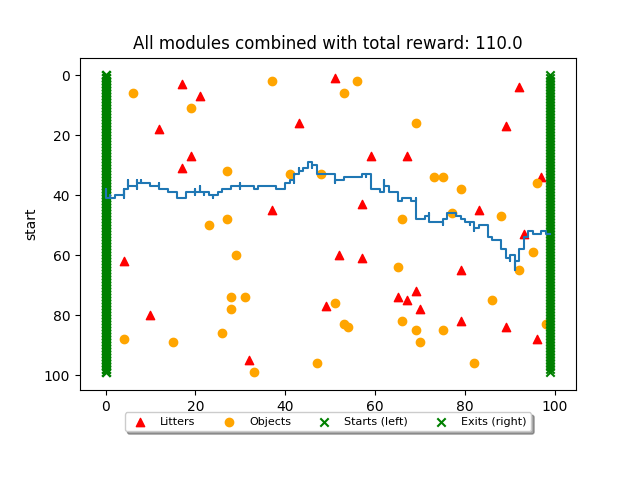
\includegraphics[scale=0.7]{combined2.png} 
\caption{Performance of all three modules combined}
\end{figure}

\begin{figure}
\centering
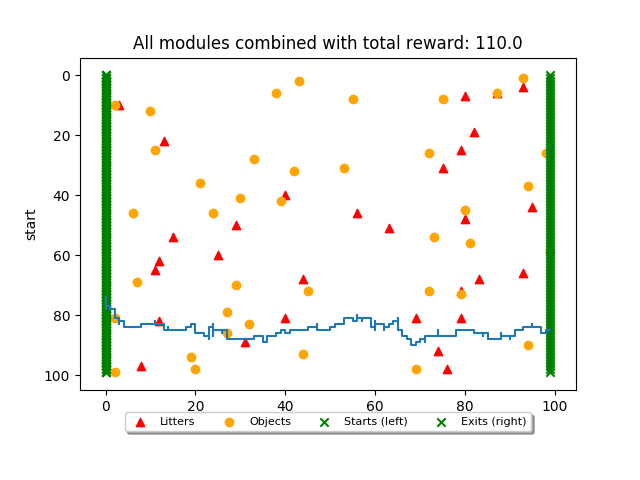
\includegraphics[scale=0.7]{combined3.png} 
\caption{Performance of all three modules combined}
\end{figure}

\begin{figure}
\centering
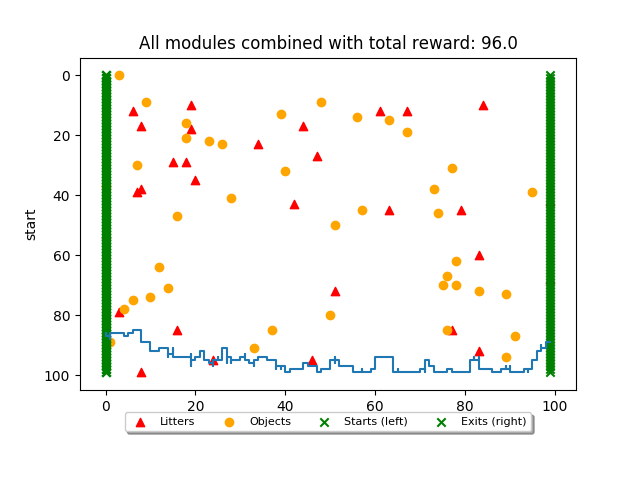
\includegraphics[scale=0.7]{combined4.png} 
\caption{Performance of all three modules combined}
\end{figure}


\end{appendices}


\end{document}
